%%%%%%%%%%%%%%%%%%%%%%%%%%%%%%%%%%%%%%%%%%%%%%%%%%%%%%%%
%GRASS PROMOTION FLYER                                 %
%(c) 2007 GRASS PROMOTION TEAM                         %
%Translated from English version by Martin Landa       %
%                              <landa.martin gmail.com>%
%GNU Free Documentation License                        %
%Version 1.2                                           %
%Needs leaflet.cls				       %
%www.ctan.org/tex-archive/macros/latex/contrib/leaflet/%
%%%%%%%%%%%%%%%%%%%%%%%%%%%%%%%%%%%%%%%%%%%%%%%%%%%%%%%%

%Sometimes printing engines need the 2nd side upside down in this
% case, use tumble (which is default) instead of notumble If this
% causes problems, use notumble If you need a foldmark, delete
% nofoldmark
\documentclass[notumble,a4paper,10pt,nofoldmark]{leaflet}
\usepackage{helvet,courier,xcolor}
\usepackage[utf8]{inputenc}

% Set Helvetica as the default font
\renewcommand*\familydefault\sfdefault
% Let LaTeX knows that pictures are found in ./pix
\graphicspath{{pix/}}

% Setting up things for the captions
\usepackage{caption}[2004/07/16]
\captionsetup{%
  font={small,it},%
  labelformat=empty,% Leaves out label: ``Figure 1''
  labelsep=none,%
  aboveskip=0pt%
}
% Defining a new 'figure' environment for the document
\newenvironment{myfig}[1][0pt plus 1.5ex minus
.5ex]{\par\vspace*{#1}\begin{minipage}{\textwidth}\centering}{\end{minipage}}

% Defining the GRASS homepage
\newcommand{\GRASSurl}{\url{http://grass.osgeo.org}}

% Define a color for the URIs
\definecolor{darkblue}{RGB}{0,0,88}

\usepackage{hyperref}
% Setting up some document info
\hypersetup{%
  colorlinks=true,%
  urlcolor=darkblue,% Redefine this color to change URIs color
  pdfauthor={GRASS Community},%
  pdftitle={GRASS GIS: Efektivita díky Svobodě \& Transparentnosti},%
  pdfsubject={GRASS propagační leták GRASS},%
  breaklinks=true,%
  plainpages=false%
}

% Title page stuff
\title{\textbf{\huge GRASS GIS}\\%
\textsl{Efektivita díky Svobodě \& Transparentnosti}}
\author{Komunita GRASSu}
\date{
\includegraphics[width=\textwidth]{grasslogo_vector}\\[2ex]
\large\GRASSurl}

\begin{document}

\maketitle
\thispagestyle{empty}% Necessary to leave out the page number on the first page

\newpage

\section{Co je GRASS}

GRASS (Geographic Resources Analysis Support System) je Svobodný/Open
Source Software určený pro prostorové analýzy. Obsahuje více než 350
modulů pro zpracování 2D/3D vektorových a rastrových dat. Nabízí řadu
rozhraní k dalším programům v dané oblasti jako je geostatistika,
databáze, mapové služby a dokonce i k dalším GIS aplikacím. Je
nej-rozsáhlejším Open Source GISem. Může sloužit jako Desktop GIS či
jako páteř kompletní GIS infrastruktury.

\section{Kde je GRASS používán}

GRASS je používán ve vědeckých aplikacích, komerčně či ve veřejné
správě po celém světě. GRASS poskytuje v mnoha případech velký
potenciál pro řešení geoprostorových úloh.

\section{Historie}

GRASS byl původně vyvíjen od počátku 80-tých let agenturou US Army
Construction Engineering Research Laboratories (USA-CERL) a byl
poskytnut jako public domain software. V okamžiku kdy USA-CERL upustil
od vývoje, vznikl mezinárodní tým vývojářů, který dál software
vyvíjí. Od roku 1999 je GRASS uvolněn jako Free Software pod licencí
GNU General Public Licence.
\begin{myfig}[1.5ex]
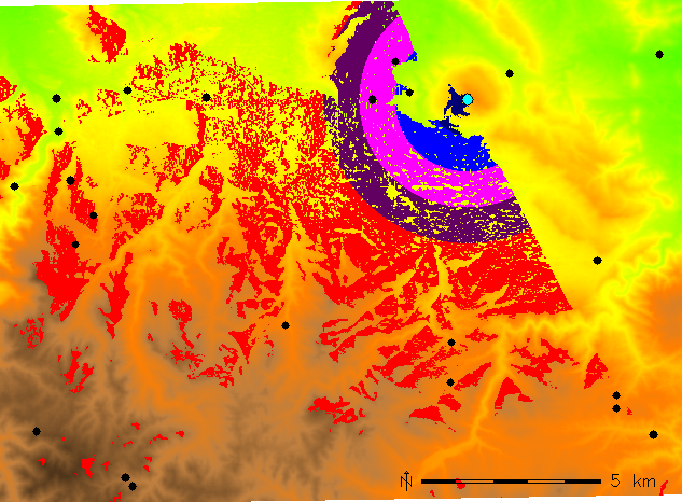
\includegraphics[width=0.7\textwidth]{visibility}
\captionof{figure}{Analýza viditelnost provedena pomocí GRASSu}
\end{myfig}

\section{Filozofie Open Source}

Filozofie Open Source nabízí uživateli možnost nahlédnutí do
zdrojových kódu a struktury programu, obrovskou míru
transparentnosti. Uživatel může rozšířit program dle svých
potřeb. Vzájemná kontrola zdrojového kódu zvyšuje jeho
kvalitu. Tzv. extension manager umožňuje vytvářet nové moduly bez
nutnosti zdrojového kódu GRASSu.

\section{Technická data}

\subsection{Licence}

Všeobecná veřejná licence GNU (GNU General Public License, Free
Software Foundation).

\subsection{Podporované platformy}

GRASS běží na téměř všech platformách. Podporuje GNU/Linux, unixové
systémy podporující Posix, MS-Windows a MacOS X.

\subsection{Design}

\begin{itemize}
\item Modulární
\item Obsahuje více než 350 modulů
\end{itemize}

\subsection{Programovací jazyky}

\begin{itemize}
\item ANSI C
\item Rozhraní GRASS- SWIG
\item Python pro WebGIS aplikace
\item Verze pro Javu: JGRASS
\end{itemize}

\subsection{Možnosti správy dat}

\begin{itemize}
\item Zpracování rastrových / vektorových / voxel dat
\item Modelování 2D / 3D rastrových / vektorových dat
\item Zpracování obrazových dat
\item Vektorová topologie / Síťové analýzy
\item Geostatistika (rozhraní pro R)
\end{itemize}

\begin{myfig}[1ex]
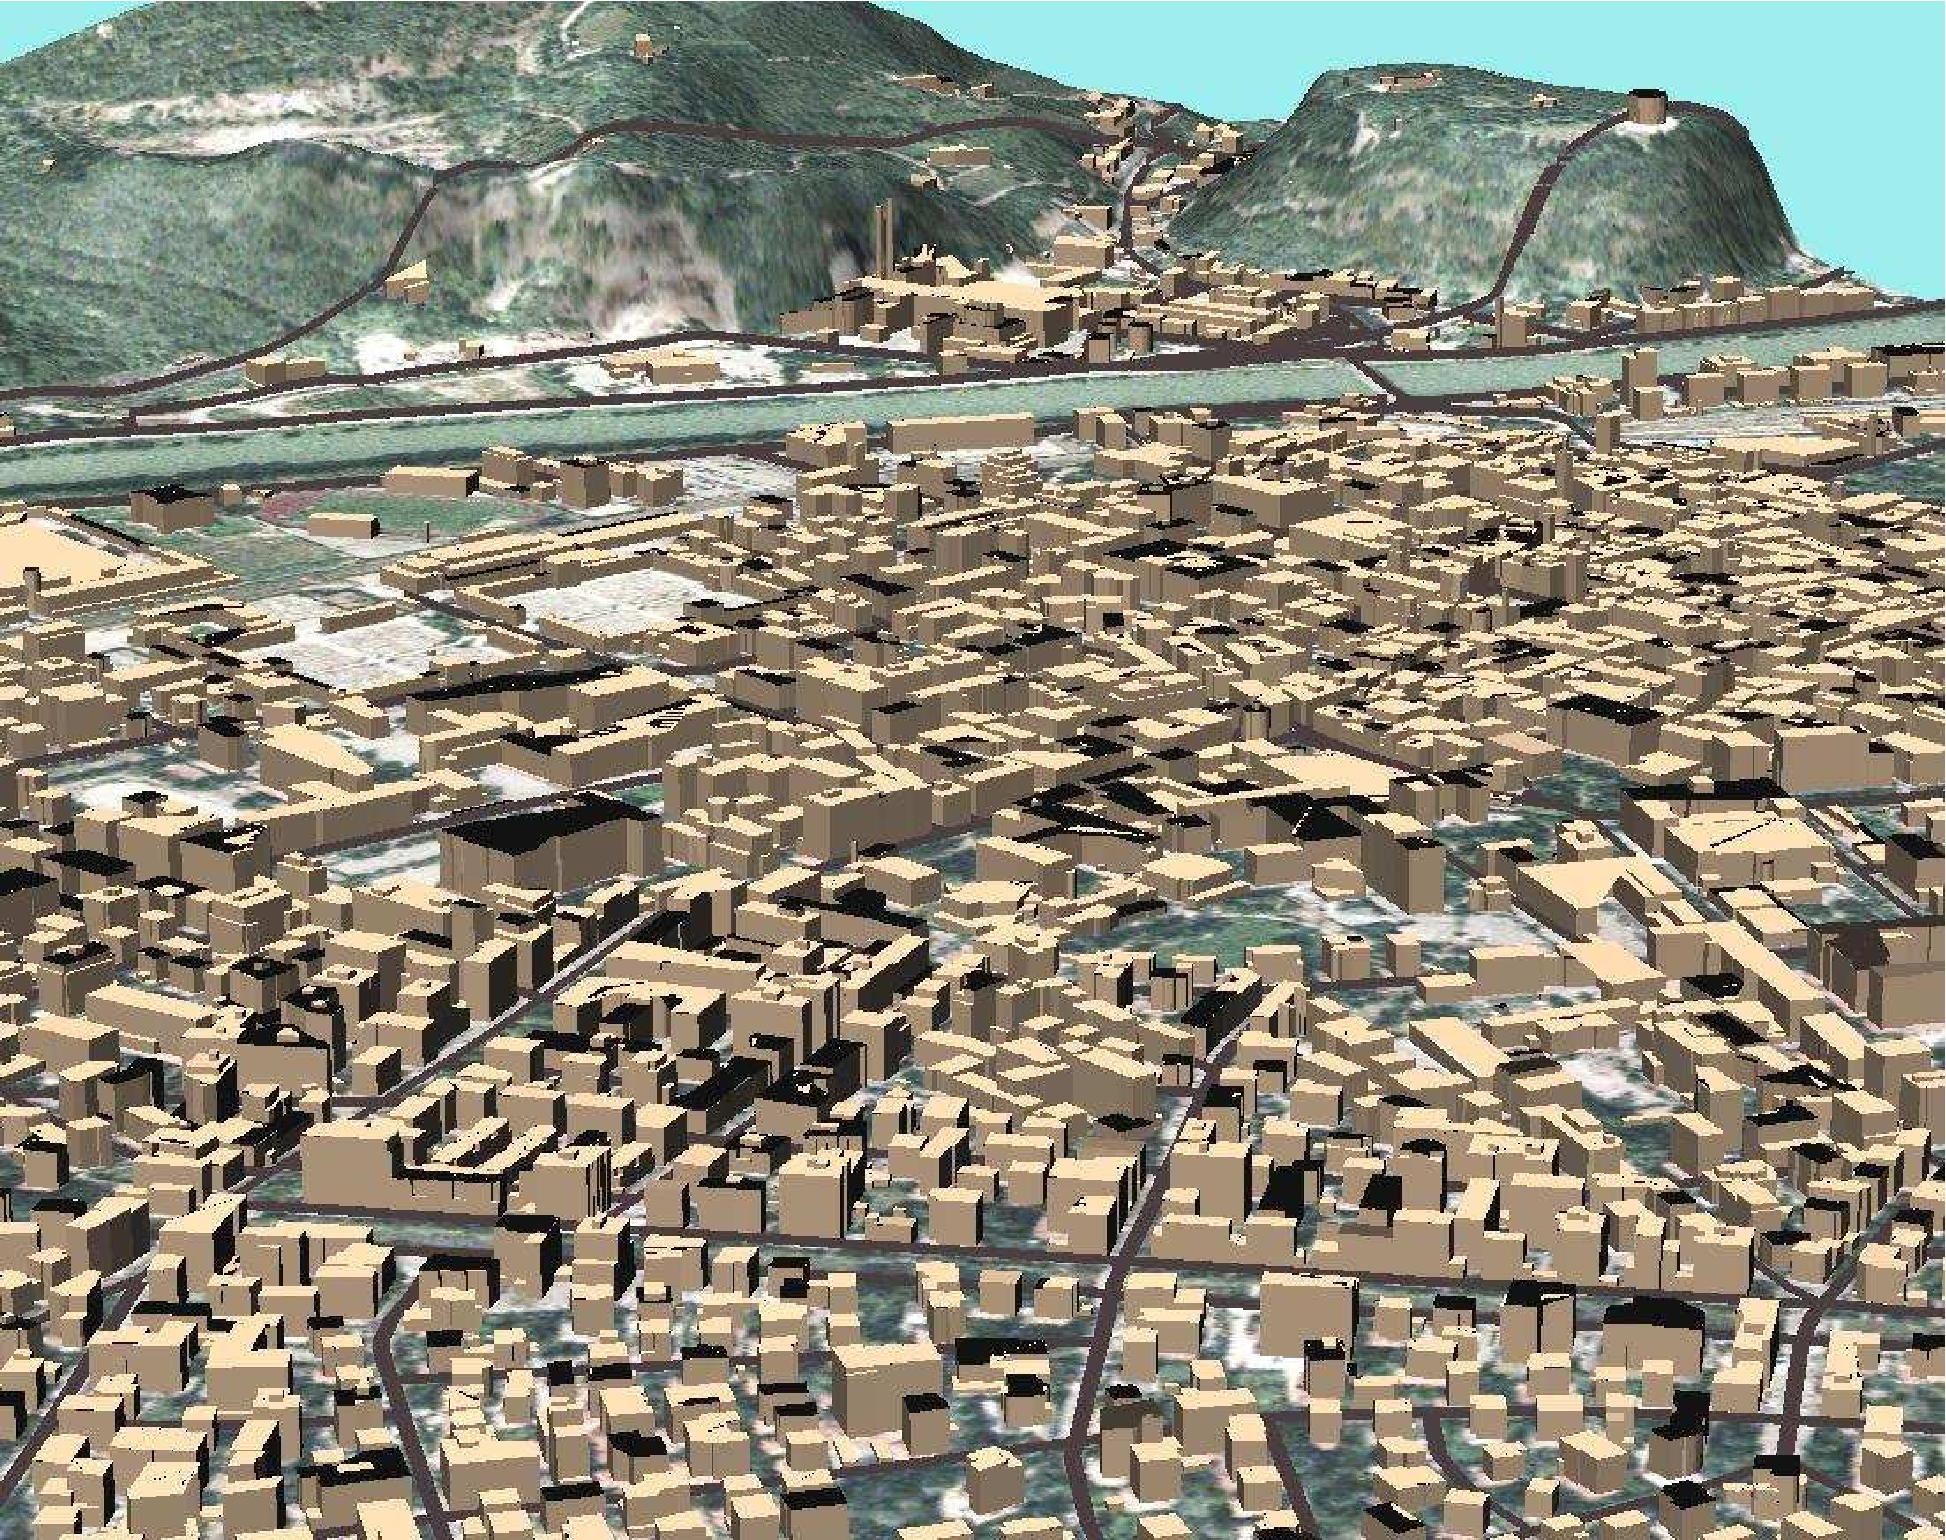
\includegraphics[width=0.7\textwidth]{trento3d}
\captionof{figure}{3D pohled na Trento, Itálie}
\end{myfig}

\section{Podporované datové formáty}

GRASS podporuje téměř všechny dobře známé GIS datové formáty díky
knihovně GDAL/OGR. Navíc podporuje Open GIS Consortium's Simple
Features.

\subsection{Vektorové datové formáty}
ASCII, ARC/INFO ungenerate, ARC/INFO E00, Arc\-View SHAPE, BIL, DLG
(U.S.), DXF, DXF3D, GMT, GPS-ASCII USGS-DEM, IDRISI, MOSS, MapInfo
MIF, TIGER, VRML, \dots

\subsection{Rastrové datové formáty}
ASCII, ARC/GRID, E00, GIF, GMT, TIF, PNG, Vis5D, SURFER (.grd),\dots
\begin{myfig}
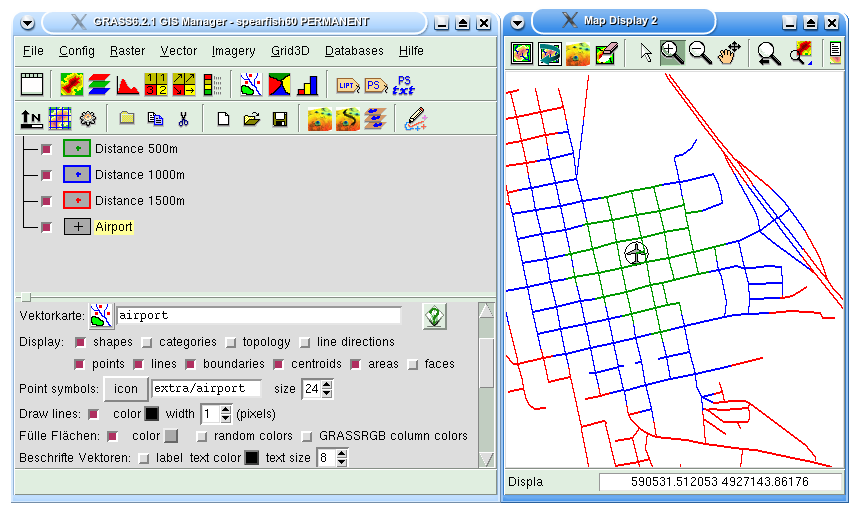
\includegraphics[width=0.7\textwidth]{isodist}
\captionof{figure}{Výchozí konfigurace GUI demonstrující možnosti
  GRASSu pro síťové analýzy}
\end{myfig}

\subsection{Obrazové datové formáty}

CEOS (SAR, SRTM, LANDSAT7 a pod.), ERDAS LAN / IMG, HDF, LANDSAT
TM/MSS, NHAP letecké snímky, SAR, SPOT, \dots
\begin{myfig}[1.5ex]
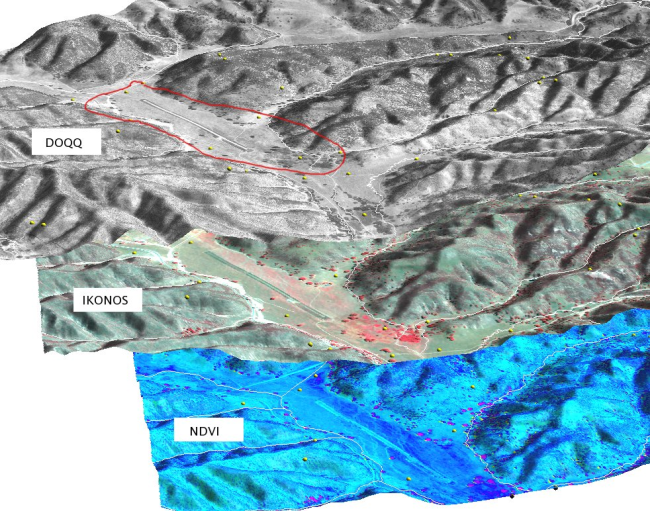
\includegraphics[width=0.7\textwidth]{ndvi}
\captionof{figure}{Možnosti GRASSu ve zpracování obrazových dat}
\end{myfig}

\subsection{Podpora databází}

\begin{itemize}
\item PostgreSQL / PostGIS
\item MySQL
\item SQLite
\item ODBC
\item DBF
\end{itemize}

\subsection{Výstup}

\begin{itemize}
\item Moduly pro tvorbu mapových výstupů
\item NVIZ pro vizualizaci 2.5D a 3D dat (tvorba animací \& pohledů)
%\item{GMT export}
%item{VRML}
\item VTK, POVray
\item WebGIS s využitím Mapserveru, Pythonu, a pod.
\end{itemize}

\subsection{Interoperabilita vůči dalším  GIS programům}

\begin{itemize}
\item Quantum GIS (Free prohlížeč geodat)
\item R- Language (statistika)
\item Gstat (geostatistika)
\item UMN Mapserver (webové služby)
\end{itemize}

\section{Kde najít další informace}

\begin{itemize}
%\begin{flushleft}
\item{Webové stránky projektu: \\\GRASSurl}
\item{GRASS Wiki: \\\url{http://grass.osgeo.org/wiki}}
\item{Propagační tým GRASSu: \\\url{malte@perlomat.de}}
\item{Elektronické konference GRASSu:
    \\\url{http://grass.osgeo.org/community/support.php}}
\item{GRASSwikiCZ: \\\url{http://grass.fsv.cvut.cz}}
\item{Elektronická konference FreeGeoCZ: \\\url{http://grass.fsv.cvut.cz/wiki/index.php/E-konference_FreeGeoCZ}}
%\end{flushleft}
\end{itemize}

\vfill
\section{OSGeo}

GRASS je zakládajícím projektem Open Source Geospatial Foundation,
která si klade za cíl tvorbu vysoce kvalitního Open Source GIS
software. Pro další informace navštivte domovskou stránku OSGeo:
\begin{center}

\includegraphics[width=0.8\textwidth]{OSGeo_CMYK}\\
\url{http://www.osgeo.org}
\end{center}

\end{document}
